\subsection{Smoothing}
In questa sezione parleremo di alcuni dei metodi che permettono di ``levigare''
le serie temporali così da poter essere successivamente analizzate.   


\subsubsection{Moving average}
In statistica, la moving average (media mobile), chiamata anche rolling mean,
è un calcolo che consente di analizzare dei dati creando una serie di 
medie di diversi sottoinsiemi dell'insieme dei dati.

Data una serie di numeri e un sottoinsieme fisso, spesso chiamato finestra (window), 
il primo elemento della media mobile si ottiene prendendo la media del sottoinsieme 
fisso iniziale della serie di numeri. 
Poi il sottoinsieme finestra viene modificato ``spostandosi in avanti'', escludendo 
il primo numero della serie e includendo il valore successivo nel sottoinsieme~\cite{wiki:roll_mean}.

Da un punto di vista matematico se consideriamo $Y$ la serie originale e $\hat{Y}$ la serie
generata dopo l'applicazione della funzione di rolling mean, e definiamo $k$ dimensione 
della finestra, numero intero positivo, le
osservazioni per ogni punto della rolling mean sono definite da
\[ \hat{y}_t = \frac{1}{k}\sum_{n = 1}^{k} y_{t-n}  \]

con $y_t$ e $\hat{y}_t$  rispettivamente osservazioni della serie originale ed osservazioni
della serie dopo l'applicazione della funzione di rolling mean, all'istante di tempo $t$.

\paragraph*{Snippet}
\begin{minted}{python3}
    def rolling_mean(serie: list | pd.Series, window: int):

        # controllo della finestra
        if window <= 0 and not isinstance(window, int):
            raise Exception('la finestra deve essere un \
                    numero intero > 0')

        # serie rolling mean
        rolling_serie: list = []

        # calcolo della rolling mean
        for i in range(len(serie) - (window-1)):

            # calcolo singolo y hat
            rolling_serie.append( np.mean(serie[i: i + (window)]) )

        return rolling_serie \
            if not isinstance(serie, pd.Series) \
            else pd.Series(
                rolling_serie, 
                index=serie.index[(window-1)//2 : -(window-1)//2])
\end{minted}

\begin{esempio}[Diversi valori per la finestra]
    Consideriamo come esempio la serie che descrive la temperatura giornaliera media
    nella città di Beijing. Se applichiamo la funzione di rolling mean con diversi
    valori per la finestra, otterremmo dei grafici come quelli mostrati in figura~\ref{fig:rolling_mean_conf}.
    
    \begin{figure}[H]
        \centering
        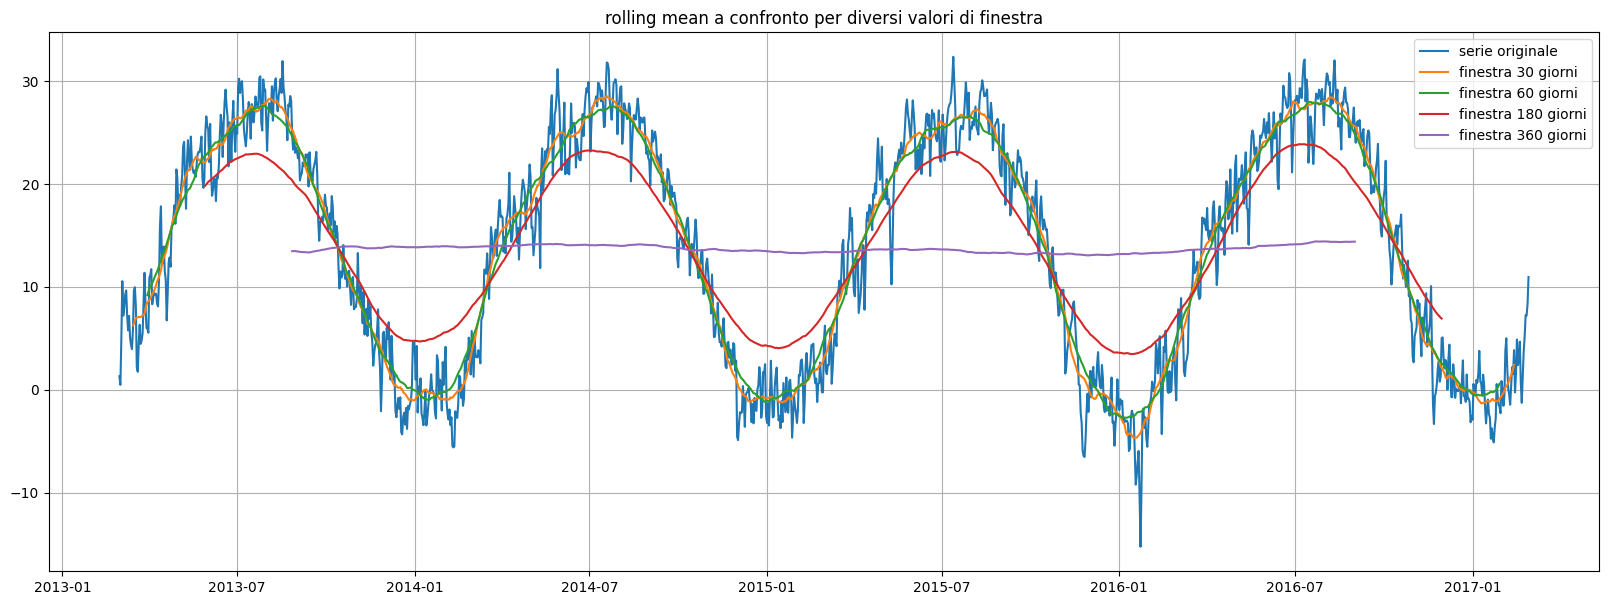
\includegraphics[width=\linewidth,keepaspectratio]{rolling_mean_conf.png}
        \caption{Funzione di rolling mean applicata a diversi valori per la finestra.}
        \label{fig:rolling_mean_conf}
    \end{figure}

\end{esempio}




\subsubsection{Exponential}
Lo smoothing esponenziale è una tecnica di regola empirica 
per ``levigare'' i dati delle serie temporali utilizzando la funzione finestra esponenziale.
Mentre nella rolling mean semplice le osservazioni passate vengono ponderate 
in modo uguale, le funzioni esponenziali vengono utilizzate per assegnare 
pesi esponenzialmente decrescenti nel tempo. 
Si tratta di una procedura di facile apprendimento e di facile applicazione 
per effettuare alcune determinazioni basate su ipotesi precedenti dell'utente, 
come la stagionalità~\cite{wiki:exp_smot}.

Da un punto di vista matematico se consideriamo $Y$ la serie originale e $\hat{Y}$ la sua 
exponential smoothing serie, dove $\hat{y}_0 = y_0$, cioè la prima osservazione
della exponential smoothing serie è inizializzata con il primo valore della serie originale,
allora le osservazioni successive per ogni punto della exponential smoothing serie
sono definite come
\[ \hat{y}_t = \alpha y_t + (1 - \alpha)\hat{y}_{t-1}  \]
con $\alpha$ numero intero positivo definito nell'intervallo $0 < \alpha < 1$,  $\hat{y}_t$
e $y_t$ rispettivamente osservazioni della exponential smoothing serie e della serie originale
all'istante di tempo $t$ definito in $t \in [1, \dots , N]$ con $N$ numero totale delle osservazioni
della serie originale.

\paragraph*{Snippet}
\begin{minted}{python3}
    def smooth_exponential(serie: list | pd.Series, alpha: float):

        # controllo per alpha
        if not isinstance(alpha, float) or alpha < 0 or alpha > 1:
            raise Exception("alpha deve essere \
                nell'intervallo 0 < alpha < 1")

        # calcolo della exponential serie
        result = [serie[0]]
        for n in range(1, len(serie)):
            result.append(
                alpha * serie[n] + (1 - alpha) * result[n - 1])

        return result \
            if not isinstance(serie, pd.Series) \
            else pd.Series(result, index=serie.index)
\end{minted}

\begin{esempio}[Diversi valori per alpha]
    Consideriamo come esempio la serie che descrive la temperatura giornaliera media
    nella città di Beijing. Se applichiamo la funzione di exponential smoothing per diversi
    valori di alpha, otterremmo dei grafici come quelli mostrati in figura~\ref{fig:exp_smoot}.
    
    \begin{figure}[H]
        \centering
        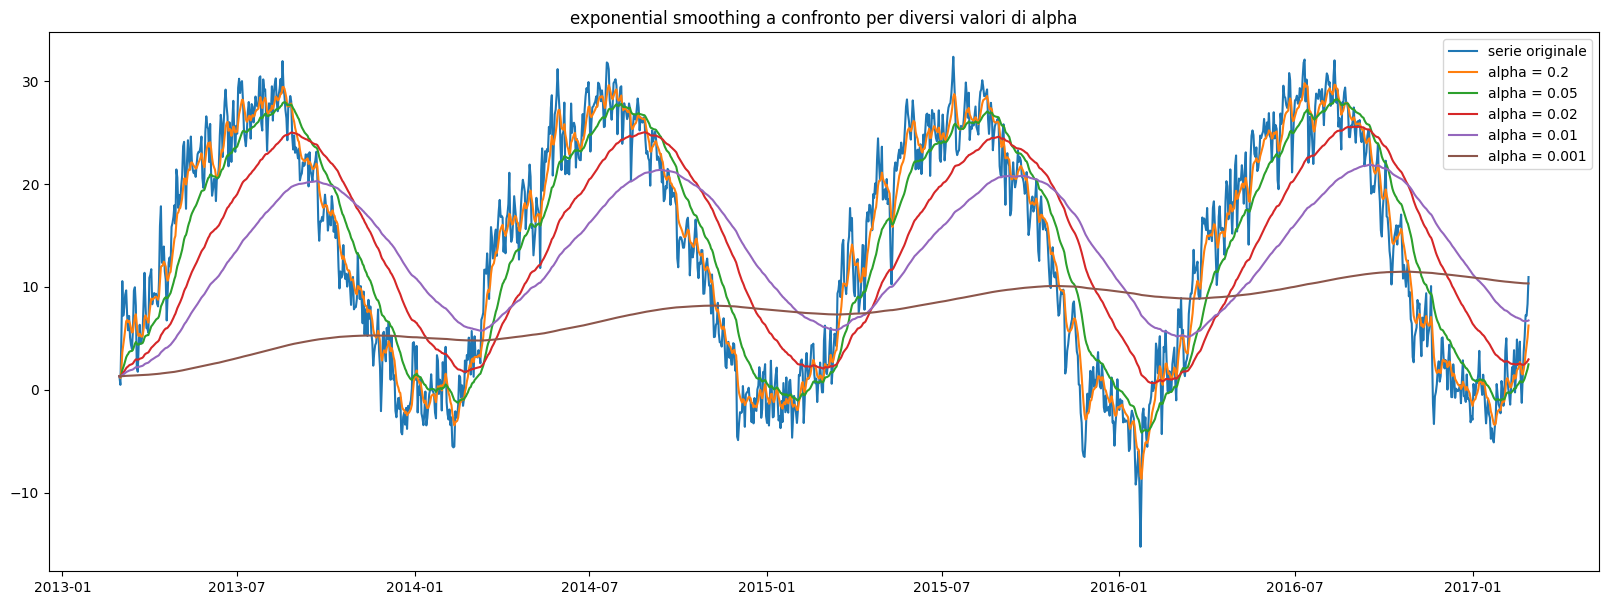
\includegraphics[width=\linewidth,keepaspectratio]{exp_smoth_conf.png}
        \caption{Funzione di exponential smoothing applicata a diversi valori di alpha.}
        \label{fig:exp_smoot}
    \end{figure}

\end{esempio}


\subsubsection{Double Exponential}
La tecnica di double exponential smoothing viene utilizzata nella previsione delle 
serie temporali quando i dati hanno una tendenza lineare (trend) ma non un andamento stagionale~\cite{si:dexp_smot}.
Questo tipo di smoothing utilizza lo stesso parametro alpha ($\alpha$) della tecnica di exponential
smoothing vista precedentemente più un ulteriore parametro beta ($\beta$) che regola l'ammontare
della componente di trend.

La decomposizione della serie ci aiuterà, quindi otteniamo così due componenti: il livello
ed il trend. Con la funzione di exponential smoothing precedente abbiamo imparato a 
prevedere il livello; ora applicheremo lo stesso exponential smoothing al trend, assumendo
che la direzione futura delle variazioni della serie temporale dipenda dalle variazioni precedenti.
Di conseguenza, otterremmo le seguenti serie di funzioni~\cite{mlc:tim_ser_an}:
\begin{align*}
    \hat{y}_0 & = y_0 \\
    \ell_0 & = y_0 \quad \\
    b_0    & = y_1 - y_0
\end{align*}
\begin{gather*}
    \ell_t = \alpha y_t + (1 - \alpha) (\ell_{t-1} + b_{t-1})\\
    b_t    = \beta(\ell_t - \ell_{t-1}) + (1 - \beta)b_{t-1} \\
    \hat{y}_{t+1} = \ell_t + b_t
\end{gather*}
dove alpha, beta sono interi positivi nell'intervallo $(0, 1)$, 
$\ell_t$ componente che regola il livello,
$b_t$ componente che regola il trend, ed infine
$\hat{y}_t$, $y_t$ rispettivamente osservazioni all'istante di tempo $t$ della double
exponential serie $\hat{Y}$ e della serie originale $Y$.

\begin{esempio}[Diversi valori per alpha]
    Consideriamo come esempio la serie che descrive la temperatura giornaliera media
    nella città di Beijing. Se applichiamo la funzione di double exponential smoothing per diversi
    valori di alpha e beta, otterremmo dei grafici come quelli mostrati 
    in figura~\ref{fig:expdoub_smoot1} e~\ref{fig:expdoub_smoot2}.
    
    \begin{figure}[H]
        \centering
        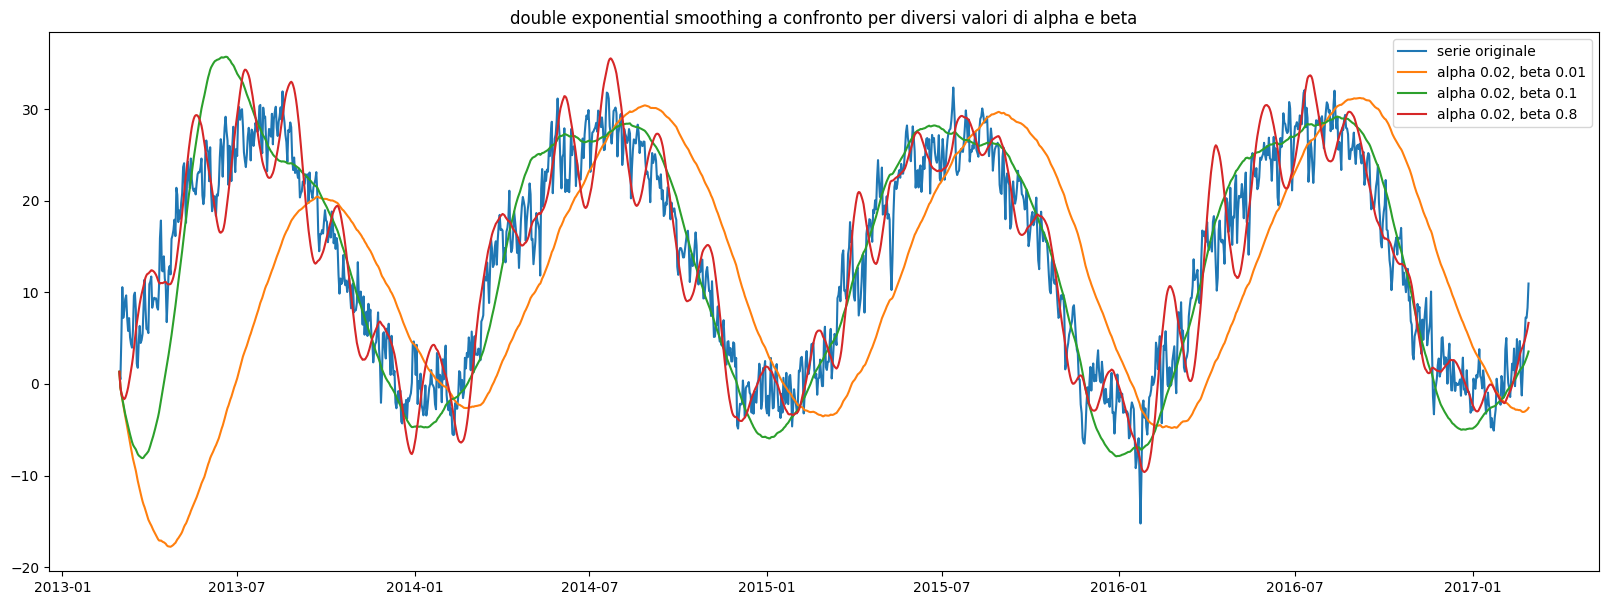
\includegraphics[width=\linewidth,keepaspectratio]{expdoub_smoth_conf1.png}
        \caption{Funzione di double exponential smoothing applicata a diversi valori di alpha e beta (alpha costante).}
        \label{fig:expdoub_smoot1}
    \end{figure}

    \begin{figure}[H]
        \centering
        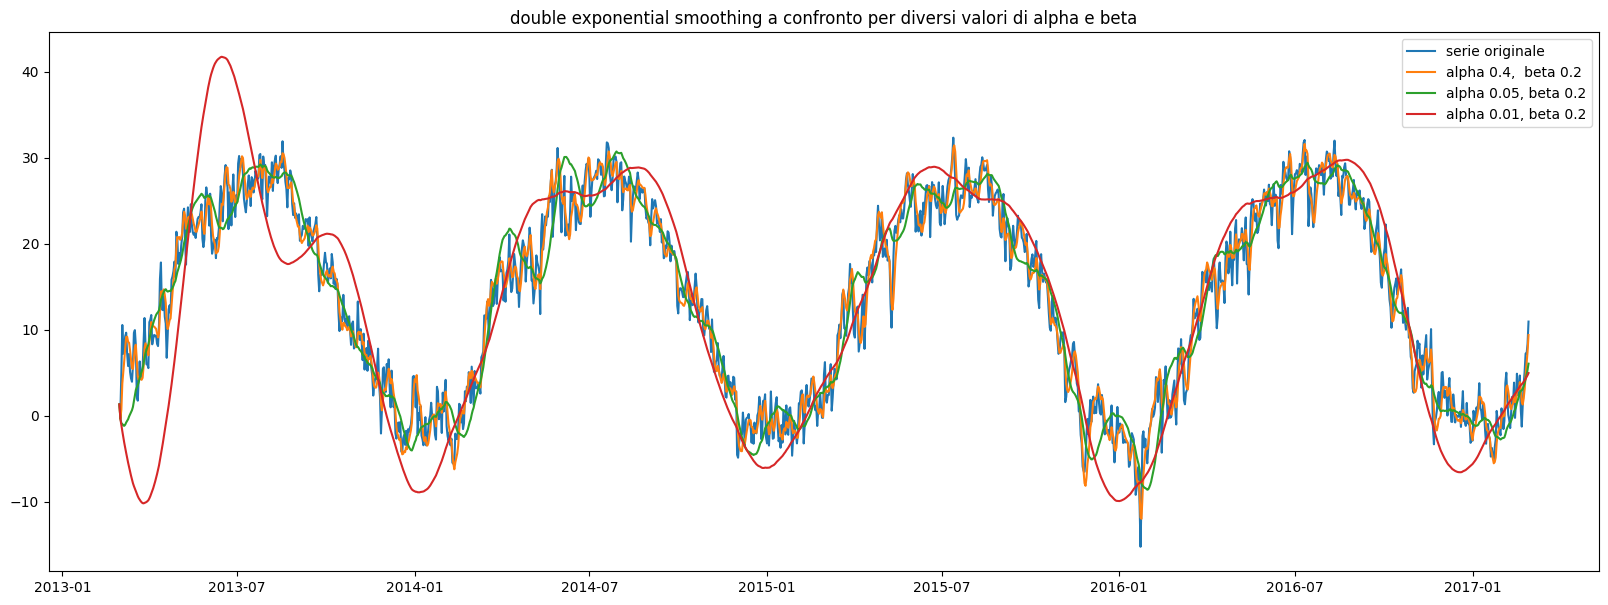
\includegraphics[width=\linewidth,keepaspectratio]{expdoub_smoth_conf2.png}
        \caption{Funzione di double exponential smoothing applicata a diversi valori di alpha e beta (beta costante).}
        \label{fig:expdoub_smoot2}
    \end{figure}

\end{esempio}